\documentclass{beamer}
\usepackage[utf8]{inputenc}

\usetheme{Madrid}
\usecolortheme{default}
\useinnertheme{circles}

\definecolor{Logo1}{rgb}{0.208, 0.2865, 0.373}
\definecolor{Logo2}{rgb}{0.000, 0.674, 0.863}

\setbeamercolor*{palette primary}{bg=Logo1, fg=white}
\setbeamercolor*{palette secondary}{bg=Logo2, fg=white}
\setbeamercolor*{palette tertiary}{bg=white, fg=Logo1}
\setbeamercolor*{palette quaternary}{bg=Logo1,fg=white}
\setbeamercolor{structure}{fg=Logo1} % itemize, enumerate, etc
\setbeamercolor{section in toc}{fg=Logo1} % TOC sections

\usepackage{graphicx,animate}
%------------------------------------------------------------
%This block of code defines the information to appear in the
%Title page
\title[Linear Algebra] %optional
{Basis \& Dimension; The Four Fundamental Subspaces}

\subtitle{Lecture 3}

\author[11910803@mail.sustech.edu.cn] % (optional)
{
    Zhang Ce
}

\institute[] % (optional)
{
    Department of Electrical and Electronic Engineering\\
    Southern University of Science and Technology
}

\date[2022.3.22] % (optional)
{2022.3.22}


%End of title page configuration block
%------------------------------------------------------------



%------------------------------------------------------------
%The next block of commands puts the table of contents at the
%beginning of each section and highlights the current section:

\AtBeginSection[]
{
\begin{frame}
    \frametitle{Table of Contents}
    \tableofcontents[currentsection]
\end{frame}
}
%------------------------------------------------------------


\begin{document}

%The next statement creates the title page.
\frame{\titlepage}


%---------------------------------------------------------
%This block of code is for the table of contents after
%the title page
\begin{frame}
\frametitle{Table of Contents}
\tableofcontents
\end{frame}
%---------------------------------------------------------
\section{A Brief Review of Last Lecture}
\begin{frame}{Last Lecture, We Discuss\dots}
Three parts in last lecture:
    \begin{enumerate}
        \item Vector Spaces and Subspaces\\
        subspaces of $\mathbb{R}^2$, higher-order subspaces
        \item Column Space and Nullspace\\
        definition and geometrical interpretation
        \item Solving Ax=0 \& Ax=b\\
        Gauss elimination; pivot column and free column; back-substitution; RREF; nullspace matrix; particular solution \& complete solution.
    \end{enumerate}
\end{frame}

\begin{frame}{Subspaces of $\mathbb{R} ^2$}
    Subspaces of $\mathbb{R} ^2$ (3 types):
    \begin{enumerate}
        \item The origin. That is the zero vector $\left[ \begin{array}{c}
            0\\
            0\\
        \end{array} \right] $.
        \item Straight lines across the origin.
        \vspace{7pt}
        \item  $\mathbb{R} ^2$ itself.
    \end{enumerate}

    \vspace{5pt}
    $\mathbb{R} ^1$ is not a subspace of $\mathbb{R} ^2$? Why?

    \vspace{3pt}
    The vectors stored in $\mathbb{R} ^1$ have only 1 component, while the vectors in $\mathbb{R} ^2$ have 2. I have to say they are quite similar because they are both lines, but they are not the same.

    \vspace{3pt}
    Try to list the subspaces of $\mathbb{R} ^5$.
\end{frame}

\begin{frame}{Associate Column Space with Linear Equation}
How about we write the solutions first, find which $b$ lead to this solution?
\begin{equation*}
    \left[ \begin{matrix}
        1&		1&		2\\
        2&		1&		3\\
        4&		1&		5\\
        7&		1&		8\\
    \end{matrix} \right] \left[ \begin{array}{c}
        x_1\\
        x_2\\
        x_3\\
    \end{array} \right] =\left[ \begin{array}{c}
        b_1\\
        b_2\\
        b_3\\
        b_4\\
    \end{array} \right]
\end{equation*}

The left side gives all possible linear combinations of the 3 column vectors.

\vspace{3pt}
You may already discover, the equation system is solvable exactly when $b$ is in $C(A)$.

\vspace{3pt}
Are these 3 column vectors \alert{linearly independent}? Or, do they all contribute to expand the dimension of column space?

\vspace{3pt}
No, because even if we delete a column, the column space will not change. We will call the linearly independent columns (contribute to column space) that come first pivot columns later.
\end{frame}

\begin{frame}{Reduced Row Echelon Form (RREF)}
Recall in Chapter 1, we can do row operations to let the matrix become an identity matirx, then the solution appears on the right side. (That is how you find the inverse of matrix.)Similarly, we can have further simplication to this linear equation system.
\begin{equation*}
    U=\left[ \begin{matrix}
        1&		3&		3&		3\\
        0&		0&		2&		4\\
        0&		0&		0&		0\\
    \end{matrix} \right] \rightarrow \left[ \begin{matrix}
        1&		3&		0&		-3\\
        0&		0&		2&		4\\
        0&		0&		0&		0\\
    \end{matrix} \right] \rightarrow \left[ \begin{matrix}
        1&		3&		0&		-3\\
        0&		0&		1&		2\\
        0&		0&		0&		0\\
    \end{matrix} \right] =R
\end{equation*}

We only do row operations, $Ax=0\Leftrightarrow Ux=0\Leftrightarrow Rx=0$.

What we have done:
\begin{itemize}
    \item Eliminate entries on the top of pivots.
    \item Make the pivots all 1.
\end{itemize}

After this process, we have the Reduced Row Echelon Form (RREF) matrix $R$. Can you discover where the solutions appear?

\vspace{3pt}
Can you find the identity matrix in $R$?

\end{frame}

\begin{frame}{Reduced Row Echelon Form (RREF)}
Let's begin with the pivot columns:
\begin{equation*}
    \left[ \begin{matrix}
        {\color[RGB]{240, 0, 0} 1}&		{\color[RGB]{240, 0, 0} 0}&		{\color[RGB]{0, 128, 255} 3}&		{\color[RGB]{0, 128, 255} -3}\\
        {\color[RGB]{240, 0, 0} 0}&		{\color[RGB]{240, 0, 0} 1}&		{\color[RGB]{0, 128, 255} 0}&		{\color[RGB]{0, 128, 255} 2}\\
        0&		0&		0&		0\\
    \end{matrix} \right]
\end{equation*}

Generally, the RREF matrices are like
\begin{equation*}
    \left[ \begin{matrix}
        {\color[RGB]{240, 0, 0} I}&		{\color[RGB]{0, 128, 255} F}\\
        0&		0\\
    \end{matrix} \right]
\end{equation*}

I repeat the solution we have solved in previous slides. Correspondingly, I write the pivot column coefficients firstly.
\begin{equation*}
    x=x_2\left[ \begin{array}{c}
        \color[RGB]{0, 128, 255} -3\\
        \color[RGB]{0, 128, 255} 0\\
        {\color[RGB]{240, 0, 0} 1}\\
        {\color[RGB]{240, 0, 0} 0}\\
    \end{array} \right] +x_4\left[ \begin{array}{c}
        \color[RGB]{0, 128, 255} 3\\
        \color[RGB]{0, 128, 255} -2\\
        {\color[RGB]{240, 0, 0} 0}\\
        {\color[RGB]{240, 0, 0} 1}\\
    \end{array} \right]
\end{equation*}

\end{frame}

\begin{frame}{Complete Solution to $Ax=b$}
How to find the complete solution? Add the particular solution by nullspace vectors!
\begin{equation*}
    Ax_p=b
\end{equation*}
\begin{equation*}
    Ax_n=0
\end{equation*}
\begin{equation*}
    A(x_p+x_n)=b
\end{equation*}

The complete solution is $x_{complete}=x_{particular}+x_{nullspace}$.

\vspace{3pt}
For our example above, the complete solution is
\begin{equation*}
    x_c=x_p+x_n=\left[ \begin{array}{c}
        -5\\
        0\\
        2\\
        0\\
    \end{array} \right] +x_2\left[ \begin{array}{c}
        -3\\
        1\\
        0\\
        0\\
    \end{array} \right] +x_4\left[ \begin{array}{c}
        3\\
        0\\
        -2\\
        1\\
    \end{array} \right], x_2, x_4 \in \mathbb{R}
\end{equation*}

Now try to understand any particular solution is OK.
\end{frame}

\begin{frame}{The Geometry of Solution Set}
Can the whole solution set construct a subspace of $\mathbb{R}^4$?

\vspace{3pt}
Firstly, let's consider nullspace only. It is a 2-dimensional plane through the origin in $\mathbb{R}^4$ space.

\vspace{3pt}
Then add a particular solution.  It is now a 2-dimensional plane away form the origin in $\mathbb{R}^4$ space.

\begin{figure}
    \centering
    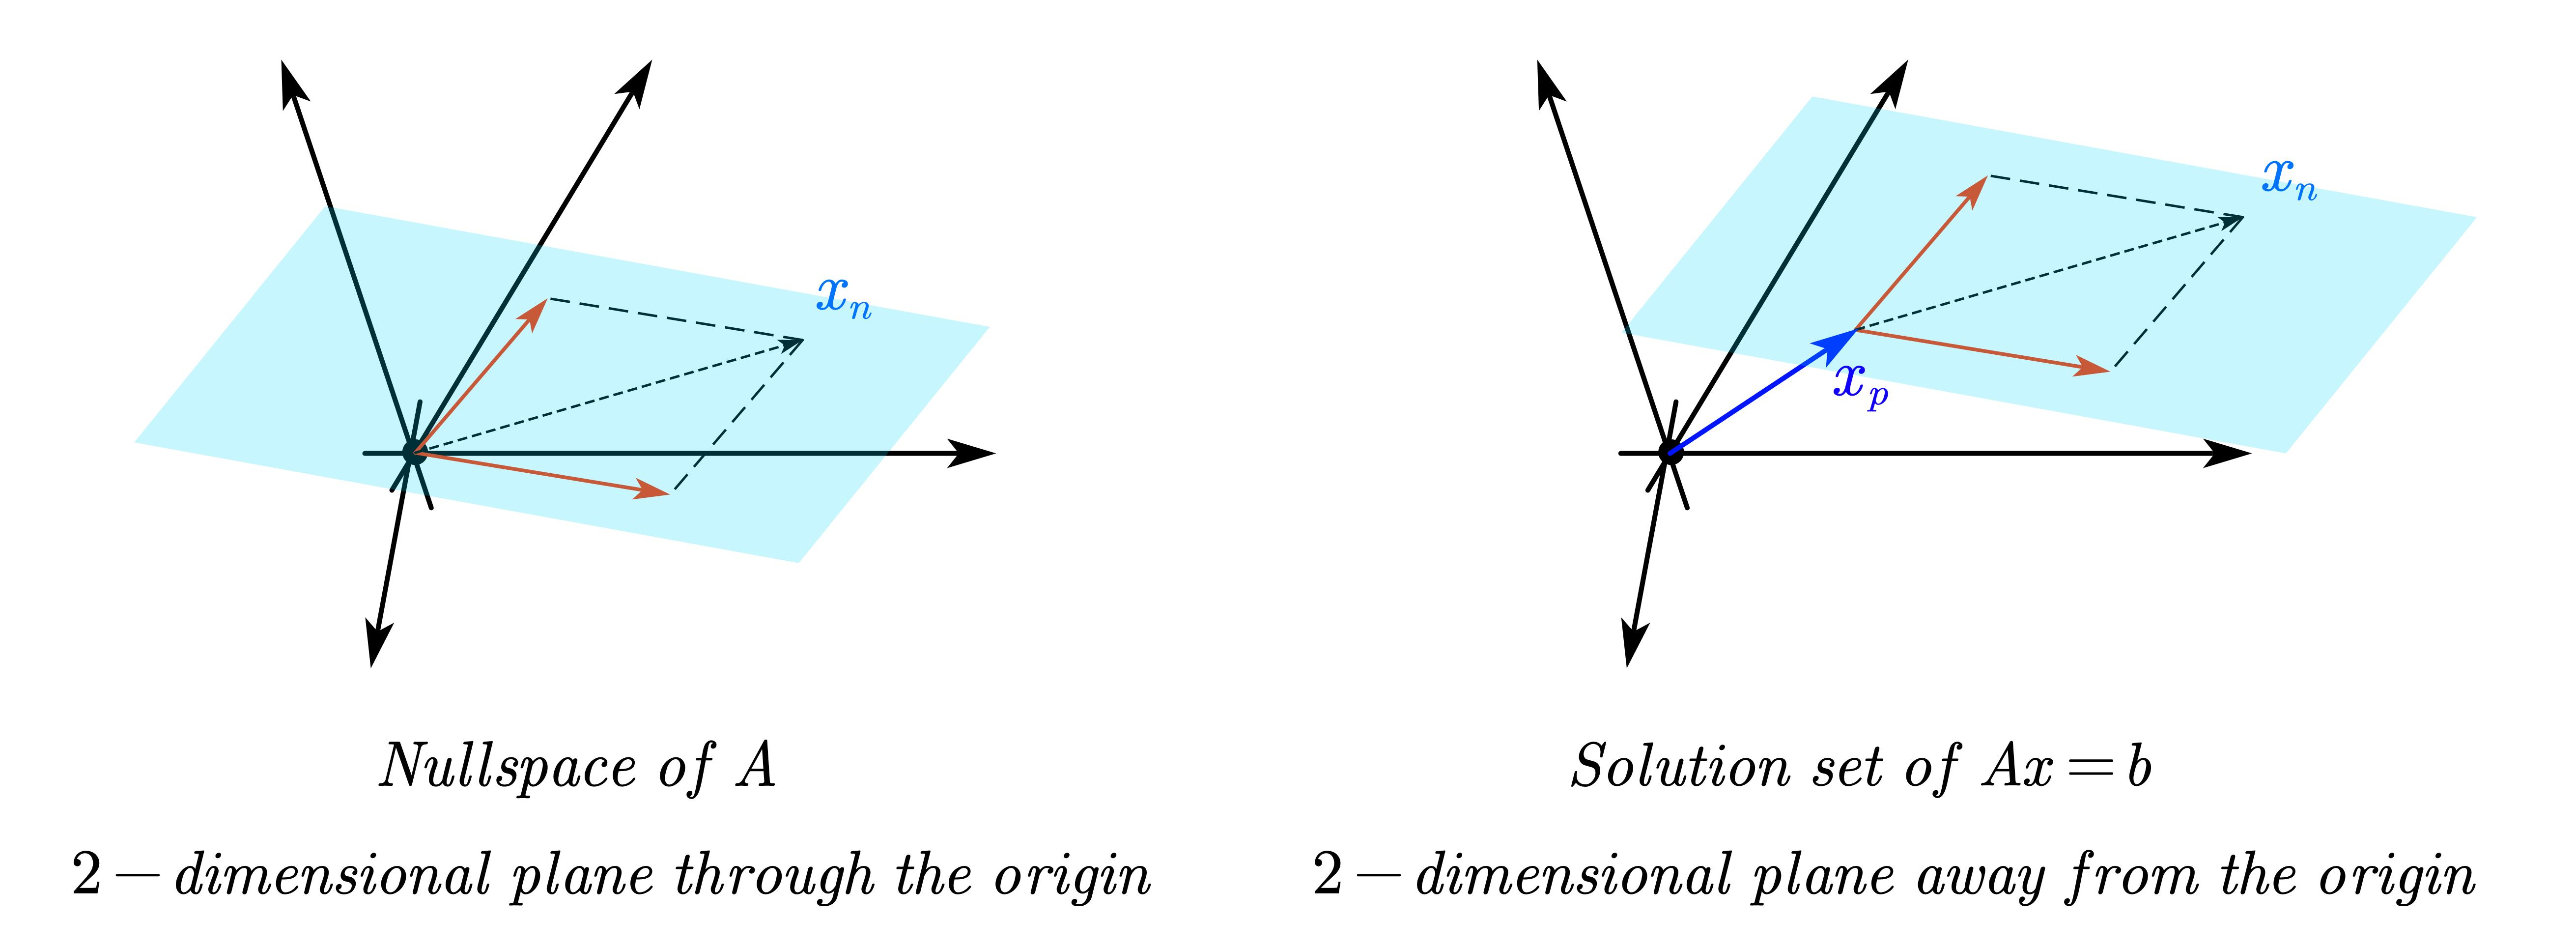
\includegraphics[width=0.9\textwidth]{sol.jpg}
\end{figure}

\end{frame}

\begin{frame}{An Important Reminder}
\begin{equation*}
    \left[ \begin{matrix}
        1&		3&		4&		2\\
        2&		7&		9&		4\\
        0&		1&		1&		0\\
    \end{matrix} \right] \rightarrow \left[ \begin{matrix}
        1&		3&		4&		2\\
        0&		1&		1&		0\\
        0&		1&		1&		0\\
    \end{matrix} \right] \rightarrow \left[ \begin{matrix}
        1&		3&		4&		2\\
        0&		1&		1&		0\\
        0&		0&		0&		0\\
    \end{matrix} \right]
\end{equation*}

After a series of row operations, the row space and the nullspace remain unchanged, but the column space changed.

\vspace{3pt}
Check if this relation of columns is still unchanged?
\begin{center}
    (Col 1) + (Col 2) = (Col 3), 2 (Col 1) = (Col 4)
\end{center}

Yes! And what is the reason behind that?

\vspace{3pt}
Because nullspace never changes! The nullspace shows us which combination of columns can lead us to zero and the relation is ever-lasting.

\vspace{3pt}
The pivot columns are the basis of $C(A)$. Try to explain that.


\end{frame}

\section{Linear Independence}
\begin{frame}{Linear Independence}
\begin{definition}
Vectors $v_1, v_2, ...$ are independent if no combination of them gives zero vector (except the zero combination $c_i=0$).
\vspace{-8pt}
\begin{equation*}
    c_1v_1+c_2v_2+...+c_nv_n\ne0
\end{equation*}
\end{definition}

Suppose $v_1=\left[ \begin{array}{c}
	1\\
	3\\
\end{array} \right], v_2=\left[ \begin{array}{c}
	2\\
	6\\
\end{array} \right]$, are they linearly independent?

No, because $2v_1-v_2=0$.

\vspace{5pt}
Suppose $v_1=\left[ \begin{array}{c}
	1\\
	3\\
\end{array} \right], v_2=\left[ \begin{array}{c}
	0\\
	0\\
\end{array} \right]$, are they linearly independent?

No, because $0v_1-6v_2=0$.

\vspace{3pt} A zero vector makes the whole set of vectors dependent because we can take zero other vectors and one zero vector to get a zero vector.
\end{frame}

\begin{frame}{Linear Independence}
Can the following 3 vectors in $\mathbb{R}^2$ be independent? Why?
\begin{equation*}
    v_1=\left[ \begin{array}{c}
        1\\
        3\\
    \end{array} \right] , v_2=\left[ \begin{array}{c}
        2\\
        1\\
    \end{array} \right] , v_3=\left[ \begin{array}{c}
        3\\
        5\\
    \end{array} \right]
\end{equation*}

We can represent every vector using 2 vectors that are not in the same line.

\vspace{3pt}
Another interpretation:
\begin{equation*}
    \left[ \begin{matrix}
        1&		2&		3\\
        3&		1&		5\\
    \end{matrix} \right] \left[ \begin{array}{c}
        c_1\\
        c_2\\
        c_3\\
    \end{array} \right] =\left[ \begin{array}{c}
        0\\
        0\\
    \end{array} \right]
\end{equation*}

This system always have nonzero solutions! Free columns always exist.

\vspace{3pt}
To repeat, if a matrix $A$ have nonzero solutions to $Ax=0$, then the columns are linearly dependent. The solution shows us which combinations of columns of $A$ gives the zero vector.
\end{frame}

\begin{frame}{Linear Independence}
\textbf{A Final Summary}:

\vspace{5pt}
Vectors $v_1, v_2, ...$ are independent if no combination of them gives zero vector (except the zero combination $c_i=0$).
\vspace{-8pt}
\begin{equation*}
    c_1v_1+c_2v_2+...\ne0
\end{equation*}

If we write the vectors in columns of $A$:
\begin{itemize}
    \item They are independent if and only if the nullspace has only the zero vector, no free columns appear and $n=r$.
    \item They are dependent if and only if the nullspace has not only the zero vector, has free columns appear and $n>r$.
\end{itemize}
\end{frame}

\section{Spanning, Basis and Dimension}
\begin{frame}{Definition of Spanning}
\begin{definition}
Vectors $v_1,v_2,...,v_n$ span a space means: the space \alert{consists of} all the combinations of these vectors.
\end{definition}

Can I use the word "contains"? No.

\vspace{3pt}
Vectors $v_1,v_2,...,v_n$ span a space means: the space is the smallest vector space that \alert{contains} all the combinations of these vectors.

\vspace{3pt}
The spanning space of a set of vectors is exactly all the combinations of the vectors.

\vspace{3pt}
The columns of $A$ span the column space $C(A)$.

\vspace{3pt}
There is no need for these vectors to be linearly independent.

\end{frame}

\begin{frame}{Definition of Basis}
\begin{definition}
Basis of a space is a set of vectors $v_1,v_2,...,v_l$ that satisfy 2 properties:
\begin{enumerate}
    \item They are independent.
    \item They span the space.
\end{enumerate}
\end{definition}

\vspace{3pt}
Find a basis for $\mathbb{R}^3$:
\begin{equation*}
    \left[ \begin{array}{c}
        1\\
        0\\
        0\\
    \end{array} \right] , \left[ \begin{array}{c}
        0\\
        1\\
        0\\
    \end{array} \right] , \left[ \begin{array}{c}
        0\\
        0\\
        1\\
    \end{array} \right]
\end{equation*}

How about the following set?
\begin{equation*}
    \left[ \begin{array}{c}
        1\\
        1\\
        2\\
    \end{array} \right] , \left[ \begin{array}{c}
        2\\
        2\\
        5\\
    \end{array} \right]
\end{equation*}

Question: Add a vector to make it a basis for $\mathbb{R}^3$.
\end{frame}

\begin{frame}{Definition of Dimension}
\begin{definition}
Basis of a space is a set of vectors $v_1,v_2,...,v_l$ that satisfy 2 properties:
\begin{enumerate}
    \item They are independent.
    \item They span the space.
\end{enumerate}
\end{definition}

Can a set of 2 vectors be a basis of $\mathbb{R}^3$?

\vspace{3pt}
No. They cannot span the space, they can only span a plane.

\vspace{3pt}
Can a set of 4 vectors be a basis of $\mathbb{R}^3$?

\vspace{3pt}
No. They cannot be independent since there always exist free columns.

\vspace{3pt}
Actually, for a particular space, the basis has the same number of vectors, and that number is called the dimension of space.
\end{frame}

\begin{frame}{Example}
Consider the matrix $A$:

\begin{equation*}
    A=\left[ \begin{matrix}
        1&		3&		4&		2\\
        2&		7&		9&		4\\
        0&		1&		1&		0\\
    \end{matrix} \right]
\end{equation*}

Can the 4 column vectors span $C(A)$?

\vspace{3pt}
Of course, it is the definition of column space.

\vspace{3pt}
But are they a basis for the column space $C(A)$?

\vspace{3pt}
No, they are not independent because $Ax=0$ has nonzero solutions.

\vspace{3pt}
Find a basis for the column space $C(A)$.

\vspace{3pt}
Column 1 and column 2. They are pivot columns also. And $dim(C(A))=2$ because one set of basis have 2 vectors.

\begin{center}
    rank $r$ $=$ \# of pivot columns = $dim(C(A))$\\
    \vspace{3pt}
    $n-r$ $=$ \# of free columns = $dim(N(A))$
\end{center}

\end{frame}

\section{The Four Fundamental Subspaces}
\begin{frame}{The Four Fundamental Subspaces}
You have known nullspace and column space before. That are 2 of the 4 fundamental subspaces.

\vspace{3pt}
The 4 fundamental subspaces are:
\begin{itemize}
    \item Column space $C(A)$
    \item Nullspace $N(A)$
    \item Row Space $C(A^T)=R(A)$
    \item Left Nullspace  $N(A^T)$
\end{itemize}

Guess the definition of Row Space and Left Nullspace...

\vspace{3pt}
Suppose we have a $m \times n$ matrix, those 4 are subspaces of ...?

\vspace{3pt}
Row space and nullspace are subspaces of $\mathbb{R}^n$; Column space and left nullspace are subspaces of $\mathbb{R}^m$.

\vspace{3pt}
What about the dimension and basis of those 4 subspaces?
\end{frame}

\begin{frame}{Review: Column Space}
Suppose a $m \times n$ matrix $A$ has rank $r$.

\vspace{3pt}
Tell me the dimension of column space $C(A)$. Explain.

\begin{center}
    rank $r$ $=$ \# of pivot columns = $dim(C(A))$
\end{center}

Tell me one basis of column space $C(A)$. Explain.

\begin{center}
    The pivot columns.
\end{center}

The pivot columns are independent and they can span the column space.
\end{frame}

\begin{frame}{Review: Nullspace}
Suppose a $m \times n$ matrix $A$ has rank $r$.

\vspace{3pt}
Tell me the dimension of column space $N(A)$. Explain.

\begin{center}
    $n-r$ $=$ \# of free columns = $dim(N(A))$
\end{center}

Tell me one basis of column space $N(A)$. Explain.

\begin{center}
    The special solutions.
\end{center}

What is the special solutions? That is the solution when we set one free variable 1, and all other free variables 0. They are also columns of nullspace matrix $N$.
\end{frame}

\begin{frame}{Row Space}
Suppose a $m \times n$ matrix $A$ has rank $r$.

\vspace{3pt}
How can I find its dimension and basis? Well, you can take transpose then find the column space.

\vspace{3pt}
Its dimension is also $r$! All the nonzero rows in $U$ or $R$ are independent and the zero rows are produced because this row can be represented by the linear combination of previous rows!

\begin{center}
    rank $r$ $=$ \# of pivots $=$ \# of nonzero rows in $U$ or $R$ $=$ $dim(R(A))$
\end{center}

And one basis...

\begin{center}
    The nonzero rows in $U$ or $R$ (not $A$).
\end{center}

How can I show that? Firstly, the number of vectors is correct, and, we can undo all the row operations to get $U$ back to $A$!
\end{frame}

\begin{frame}{An Example}
Consider matrix $A$:
\begin{equation*}
    \left[ \begin{matrix}
        1&		3&		4&		2\\
        2&		7&		9&		4\\
        0&		1&		1&		0\\
    \end{matrix} \right] \rightarrow \left[ \begin{matrix}
        1&		3&		4&		2\\
        0&		1&		1&		0\\
        0&		1&		1&		0\\
    \end{matrix} \right] \rightarrow \left[ \begin{matrix}
        1&		3&		4&		2\\
        0&		1&		1&		0\\
        0&		0&		0&		0\\
    \end{matrix} \right] \rightarrow \left[ \begin{matrix}
        1&		0&		1&		2\\
        0&		1&		1&		0\\
        0&		0&		0&		0\\
    \end{matrix} \right]
\end{equation*}

Find the dimension and a basis for $C(A), N(A), C(A^T)$.

\vspace{3pt}
The dimensions are 2, 2, 2.

\begin{equation*}
    C\left( A \right) :\left[ \begin{array}{c}
        1\\
        2\\
        0\\
    \end{array} \right] ,\left[ \begin{array}{c}
        3\\
        7\\
        1\\
    \end{array} \right] \,\, N\left( A \right) :\left[ \begin{array}{c}
        -1\\
        -1\\
        1\\
        0\\
    \end{array} \right] ,\left[ \begin{array}{c}
        -2\\
        0\\
        0\\
        1\\
    \end{array} \right] \,\,C\left( A^T \right) :\left[ \begin{array}{c}
        1\\
        0\\
        1\\
        2\\
    \end{array} \right] ,\left[ \begin{array}{c}
        0\\
        1\\
        1\\
        0\\
    \end{array} \right]
\end{equation*}
\end{frame}

\begin{frame}{Left Nullspace}
Suppose a $m \times n$ matrix $A$ has rank $r$.

\vspace{3pt}
Guess the dimension of this subspace. $m-r$. The transpose of $A$ has $m$ columns.

\vspace{3pt}
How to find a basis? Transpose the matrix and find the basis of nullspace is exactly a good way. But any other methods?

\vspace{3pt}
We look for which combination of rows makes the zero rows. The method is: trace the operations of rows, represent it by matrix $E$.

\vspace{3pt}
Which matrix $E$ makes $EA=R$?

\begin{equation*}
    \left[ \begin{matrix}
        A&		I\\
    \end{matrix} \right] \xrightarrow[E]{row\,\,operations}\left[ \begin{matrix}
        R&		E\\
    \end{matrix} \right]
\end{equation*}
\end{frame}

\begin{frame}{An Example}
Consider matrix $A$:
\begin{equation*}
    \left[ \begin{matrix}
        1&		3&		4&		2\\
        2&		7&		9&		4\\
        0&		1&		1&		0\\
    \end{matrix} \right] \rightarrow \left[ \begin{matrix}
        1&		0&		1&		2\\
        0&		1&		1&		0\\
        0&		0&		0&		0\\
    \end{matrix} \right]
\end{equation*}

Find the dimension and a basis for $N(A^T)$.

\vspace{3pt}
The dimension is 1.

\begin{equation*}
    \left[ \begin{matrix}
        1&		3&		4&		2&		1&		0&		0\\
        2&		7&		9&		4&		0&		1&		0\\
        0&		1&		1&		0&		0&		0&		1\\
    \end{matrix} \right] \rightarrow \left[ \begin{matrix}
        1&		3&		4&		2&		1&		0&		0\\
        0&		1&		1&		0&		-2&		1&		0\\
        0&		0&		0&		0&		2&		-1&		1\\
    \end{matrix} \right]
\end{equation*}

\begin{equation*}
    \left[ \begin{matrix}
        1&		0&		0\\
        -2&		1&		0\\
        2&		-1&		1\\
    \end{matrix} \right] \left[ \begin{matrix}
        1&		3&		4&		2\\
        2&		7&		9&		4\\
        0&		1&		1&		0\\
    \end{matrix} \right] =\left[ \begin{matrix}
        1&		3&		4&		2\\
        0&		1&		1&		0\\
        0&		0&		0&		0\\
    \end{matrix} \right]
\end{equation*}

A basis: $\left[ \begin{matrix}
	2&		-1&		1\\
\end{matrix} \right] ^T$. We find all basis without $A^T$!
\end{frame}

\begin{frame}{The Whole Picture of 4 Fundamental Subspaces}
\begin{center}
    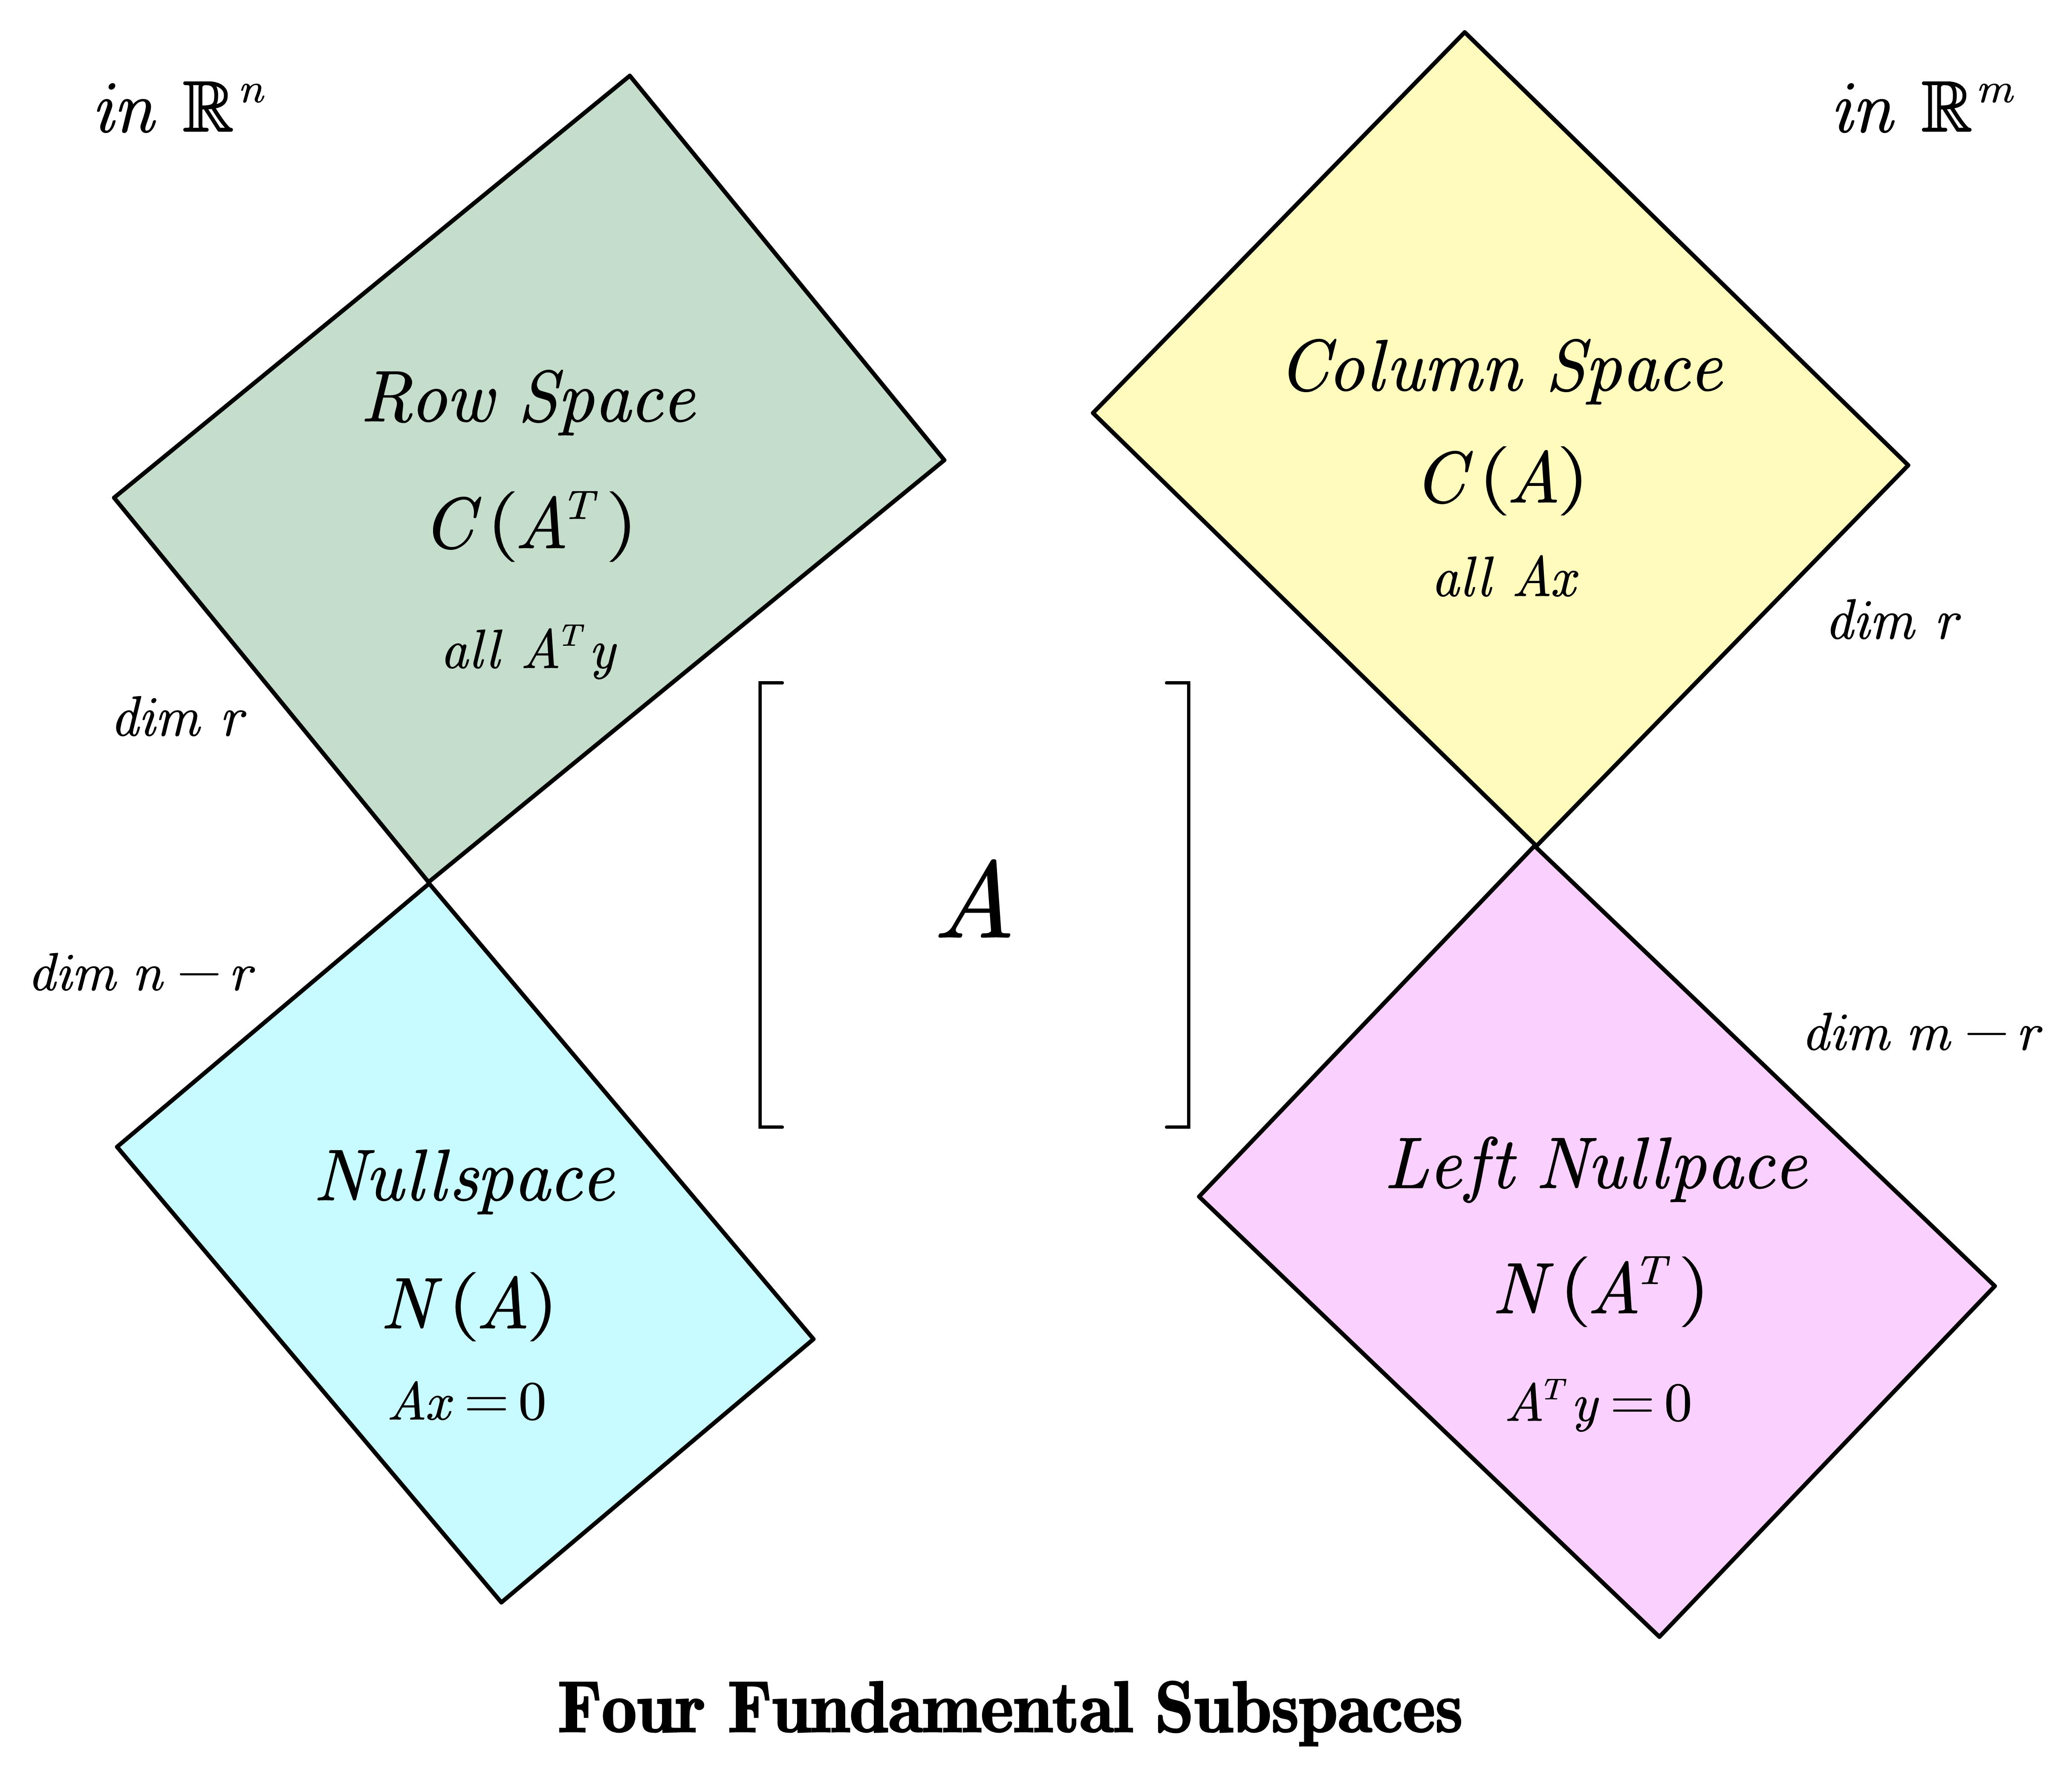
\includegraphics[width=0.74\textwidth]{subspace.jpg}
\end{center}
\end{frame}
\end{document}